% ----------------------------------------------------------------------
%  Pracovní úkoly
% ----------------------------------------------------------------------
\section{Pracovní úkoly}

\begin{enumerate}
\item Změřte teplotní závislost povrchového napětí destilované vody $\sigma$ v rozsahu teplot od 23°C do 70°C metodou bublin.

\item Měřenou závislost znázorněte graficky, do grafu vyneste chybové úsečky a tabulkové hodnoty. Závislost aproximujte kvadratickou funkcí.

\end{enumerate}

% ----------------------------------------------------------------------
%  Teoretická část
% ----------------------------------------------------------------------
\section{Teoretická část}

Na obrázku \ref{fig:aparatura-povrchove-napeti} je znázorněna aparatura pro měření závislosti povrchového napětí na teplotě podle [1].

\begin{figure}[h]
    \centering
    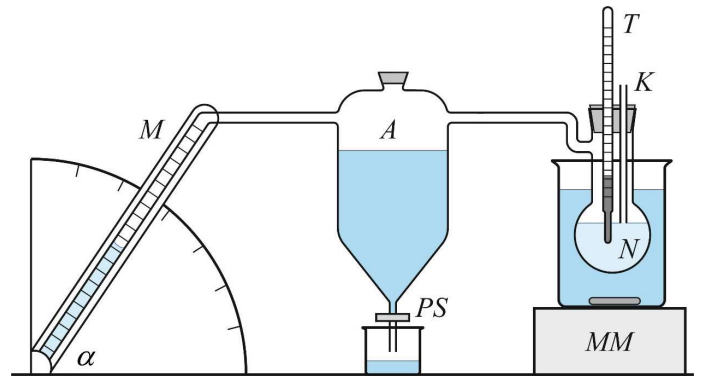
\includegraphics[width=0.75\linewidth]{14 - Studium teplotní závislosti povrchového napětí//Protokol - studium povrchového napětí//img/Aparatura.png}
    \caption{Aparatura pro měření povrchového napětí}
    \label{fig:aparatura-povrchove-napeti}
\end{figure}

Měřená kapalina se nachází v nádobce N. Do této nádoby je zavedena kapilára K, která je spojena s vnějším prostorem. Je ponořena těsně pod hladinu a my tak můžeme zanedbat hydrostatický tlak kapaliny působící na konec této trubice. V aspirátoru A je umístěna voda jejíž odtok lze regulovat přítlačnou svorkou PS. Prostor nad kapalinou je propojen se uzavřenou nádobou N a mikromanometrem M, který umožňuje měřit rozdíl tlaku. Aspirátor funguje na principu vodní vývěvy a tím snižuje tlak oproti tlaku ve vnějším prostoru. Díky tomuto rozdílu tlaků se u kapiláry začne vytvářet bublinka, až se nakonec oddělí a zvýší zpět tlak v prostoru nad hladinou.

Na vytlačovaná vzduch z kapiláry tedy působí hydrostatický tlak, který můžeme zanedbat a povrchové napětí napětí kapaliny $\sigma$. Uvnitř kulové plochy o poloměru $r$ se vytváří kapilární přetlak $\Delta p_\sigma$

\begin{equation}
    \Delta p_\sigma = \frac{2\sigma}{r}
\end{equation}

Tento přetlak je největší ve chvíli, kdy je poloměr $r$ bubliny nejmenší, tedy shodný s poloměrem kapiláry.

Pro určení tlakového rozdílu použijeme vztah

\begin{equation}
    \Delta p = d \rho g \sin{\alpha}
\end{equation}

kde $d$ je výška vodního sloupce v mikromanometru, $g$ tíhové zrychlení, $\rho$ je hustota kapaliny v mikromanometru a $\sin{\alpha}$ úhel sklonu mimkomanometrické trubice.

V našem případě je skol trubice 30° a můžeme tedy dosadit

\begin{equation}
    \sin{30^{\circ}} = \frac{1}{2}
\end{equation}

Uvažujeme maximální povrchové napětí a společně s (1) dostáváme

\begin{equation}
    \sigma = \frac{1}{4} d_{max} \rho g r
\end{equation}

kde $d_{max}$ je maximální výška hladiny v mikromanometru a $r$ poloměr trubice.

% ----------------------------------------------------------------------
%  Výsledky a zpracování měření
% ----------------------------------------------------------------------
\section{Výsledky a zpracování měření}

\subsection{Laboratorní podmínky}

    Měření bylo prováděno za laboratorních podmínek uvedených v tabulce \ref{tab:lab_pod}.

    \begin{table}[h]
        \centering
        \begin{tabular}{|c|c|c|} 
        \hline
            t / °C & p / hPa & vlhkost / \%RH  \\ 
        \hline
            24,3(4)   & 983,2(20)   & 38,9(25)            \\
        \hline
        \end{tabular}
        \caption{Laboratorní podmínky}
        \label{tab:lab_pod}
    \end{table}

\subsection{Měření povrchového napětí}

Do nádoby N je vložen teploměr pomocí kterého budeme odečítat teploty měřené kapaliny. Uvažujeme tedy maximální kapilární přetlak, proto odečítáme maximální výšku $d$ v mikromanometru za dané teploty. Na začátku, kdy má měřená destilovaná voda laboratorní teplotu, změříme povrchové napětí třikrát pro určení nejistoty typu A. Tato měření jsou znázorněna a vyhodnocena v tabulce \ref{tab:nejistota-A}.

\begin{table}[h]
\centering
\begin{tabular}{|c|cc|}
\hline
Číslo měření        & \multicolumn{1}{c|}{d / mm} & \sigma / 10^{-3} N/m \\ \hline
1                   & \multicolumn{1}{c|}{109}    & 69,31              \\ \hline
2                   & \multicolumn{1}{c|}{108}    & 68,68              \\ \hline
3                   & \multicolumn{1}{c|}{109}    & 69,31              \\ \hline
Aritmetický průměr  &                             & 69,10              \\ \hline
Směrodatná odchylka &                             & 0,04               \\ \hline
\end{tabular}
\caption{Měření nejistoty typu A}
\label{tab:nejistota-A}
\end{table}

kde směrodatná odchylka je rovna nejistotě typu A, kterou označíme $\psi_A$.

Poté jsme zapnuli zahřívání a průběžně zaznamenávali výšku $d$ při stoupající teplotě. Rovnoměrné zahřívání zajišťovalo magnetické míchátko. V tabulce \ref{tab:napeti-na-teplote} jsou zaznamenaná jednotlivá měření.

\begin{table}[h]
\centering
\begin{tabular}{|c|c|c|c|c|}
\hline
Teplota /  °C & d / mm & \sigma / 10^{-3} N/m & \psi_{\sigma} / 10^{-3} N/m & \psi / 10^{-3} N/m \\ \hline
24            & 109    & 69,31            & 2,74        & 2,74 \\ \hline
25            & 106    & 67,40            & 2,67        & 2,67 \\ \hline
27            & 105    & 66,77            & 2,65        & 2,65 \\ \hline
30            & 103    & 65,50            & 2,60        & 2,60 \\ \hline
33            & 101    & 64,23            & 2,55        & 2,55 \\ \hline
37            & 100    & 63,59            & 2,53        & 2,53 \\ \hline
40            & 99     & 62,95            & 2,50        & 2,50 \\ \hline
45            & 98     & 62,32            & 2,48        & 2,48 \\ \hline
48            & 97     & 61,68            & 2,46        & 2,46 \\ \hline
50,5          & 96     & 61,05            & 2,43        & 2,43 \\ \hline
55            & 95     & 60,41            & 2,41        & 2,41 \\ \hline
58            & 94     & 59,77            & 2,39        & 2,39 \\ \hline
60,5          & 94     & 59,77            & 2,39        & 2,39 \\ \hline
65            & 93     & 59,14            & 2,36        & 2,36 \\ \hline
68            & 92     & 58,50            & 2,34        & 2,34 \\ \hline
70            & 92     & 58,50            & 2,34        & 2,34 \\ \hline
\end{tabular}
\caption{Měření závislosti povrchového napětí na teplotě}
\label{tab:napeti-na-teplote}
\end{table}

kde $\sigma$ je spočtena podle (4). Jako hodnota $g$ bylo uvažováno $g = 9,81 \; m \cdot s^{-2}$ podle [3]. \newline Hustota $\rho = 997,249 \; kg / m^3$ při laboratorní teplotě $24,2 \; ^\circ C$.

Chyba teploty $\psi_T$ je odhadnuta jako polovina nejmenšího dílku, tedy $\psi_T = 0,5 \; ^\circ C$.

$\psi_{\sigma}$ je nejistota typu B jednotlivých měření. Je určena pomocí zákonu přenosu chyb

\begin{equation}
    \sigma^2 = \sum_{i=1}^{N} \left( \frac{\partial f}{\partial x_i} \right)^2 \sigma^2_{x_i}
\end{equation}

\newpage

odtud dostáváme

\begin{equation}
    \psi_{\sigma} = \sigma \sqrt{\left( \frac{\psi_d}{d} \right)^2 + \left( \frac{\psi_r}{r} \right)^2}
\end{equation}

kde $\psi_d$ je chyba výšky vodního sloupce a $\psi_r$ je chyba poloměru kapiláry. Chyba $\psi_r$ je zadána ve studijním textu jako $\psi_r$ = 0,01 mm a chyba $\psi_d$ byla určena jako jeden dílek na stupnici, tedy $\psi_d$ = 1 mm. Tato hodnota byla odhadnuta jako polovina nejmenšího dílku a navíc nadhodnocena, protože trubice je nakloněna a meniskus kapaliny také může ztížit čitelnost.

Pro přehlednost můžeme dosadit a nejistotu $\psi_\sigma$ vyjádřit jako

\begin{equation}
    \psi_\sigma = \sigma \sqrt{\frac{1}{d^2} + \left( \frac{0,01}{0,26} \right)^2}
\end{equation}

kde za $d$ dosazujeme v milimetrech.

Celková nejistota $\psi$ je spočtena jako

\begin{equation}
    \psi = \sqrt{\psi^2_A + \psi^2_{\sigma}}
\end{equation}

Tuto závislost můžeme zanést do grafu \ref{fig:napeti-na-teplote}.

\begin{figure}[h]
    \centering
    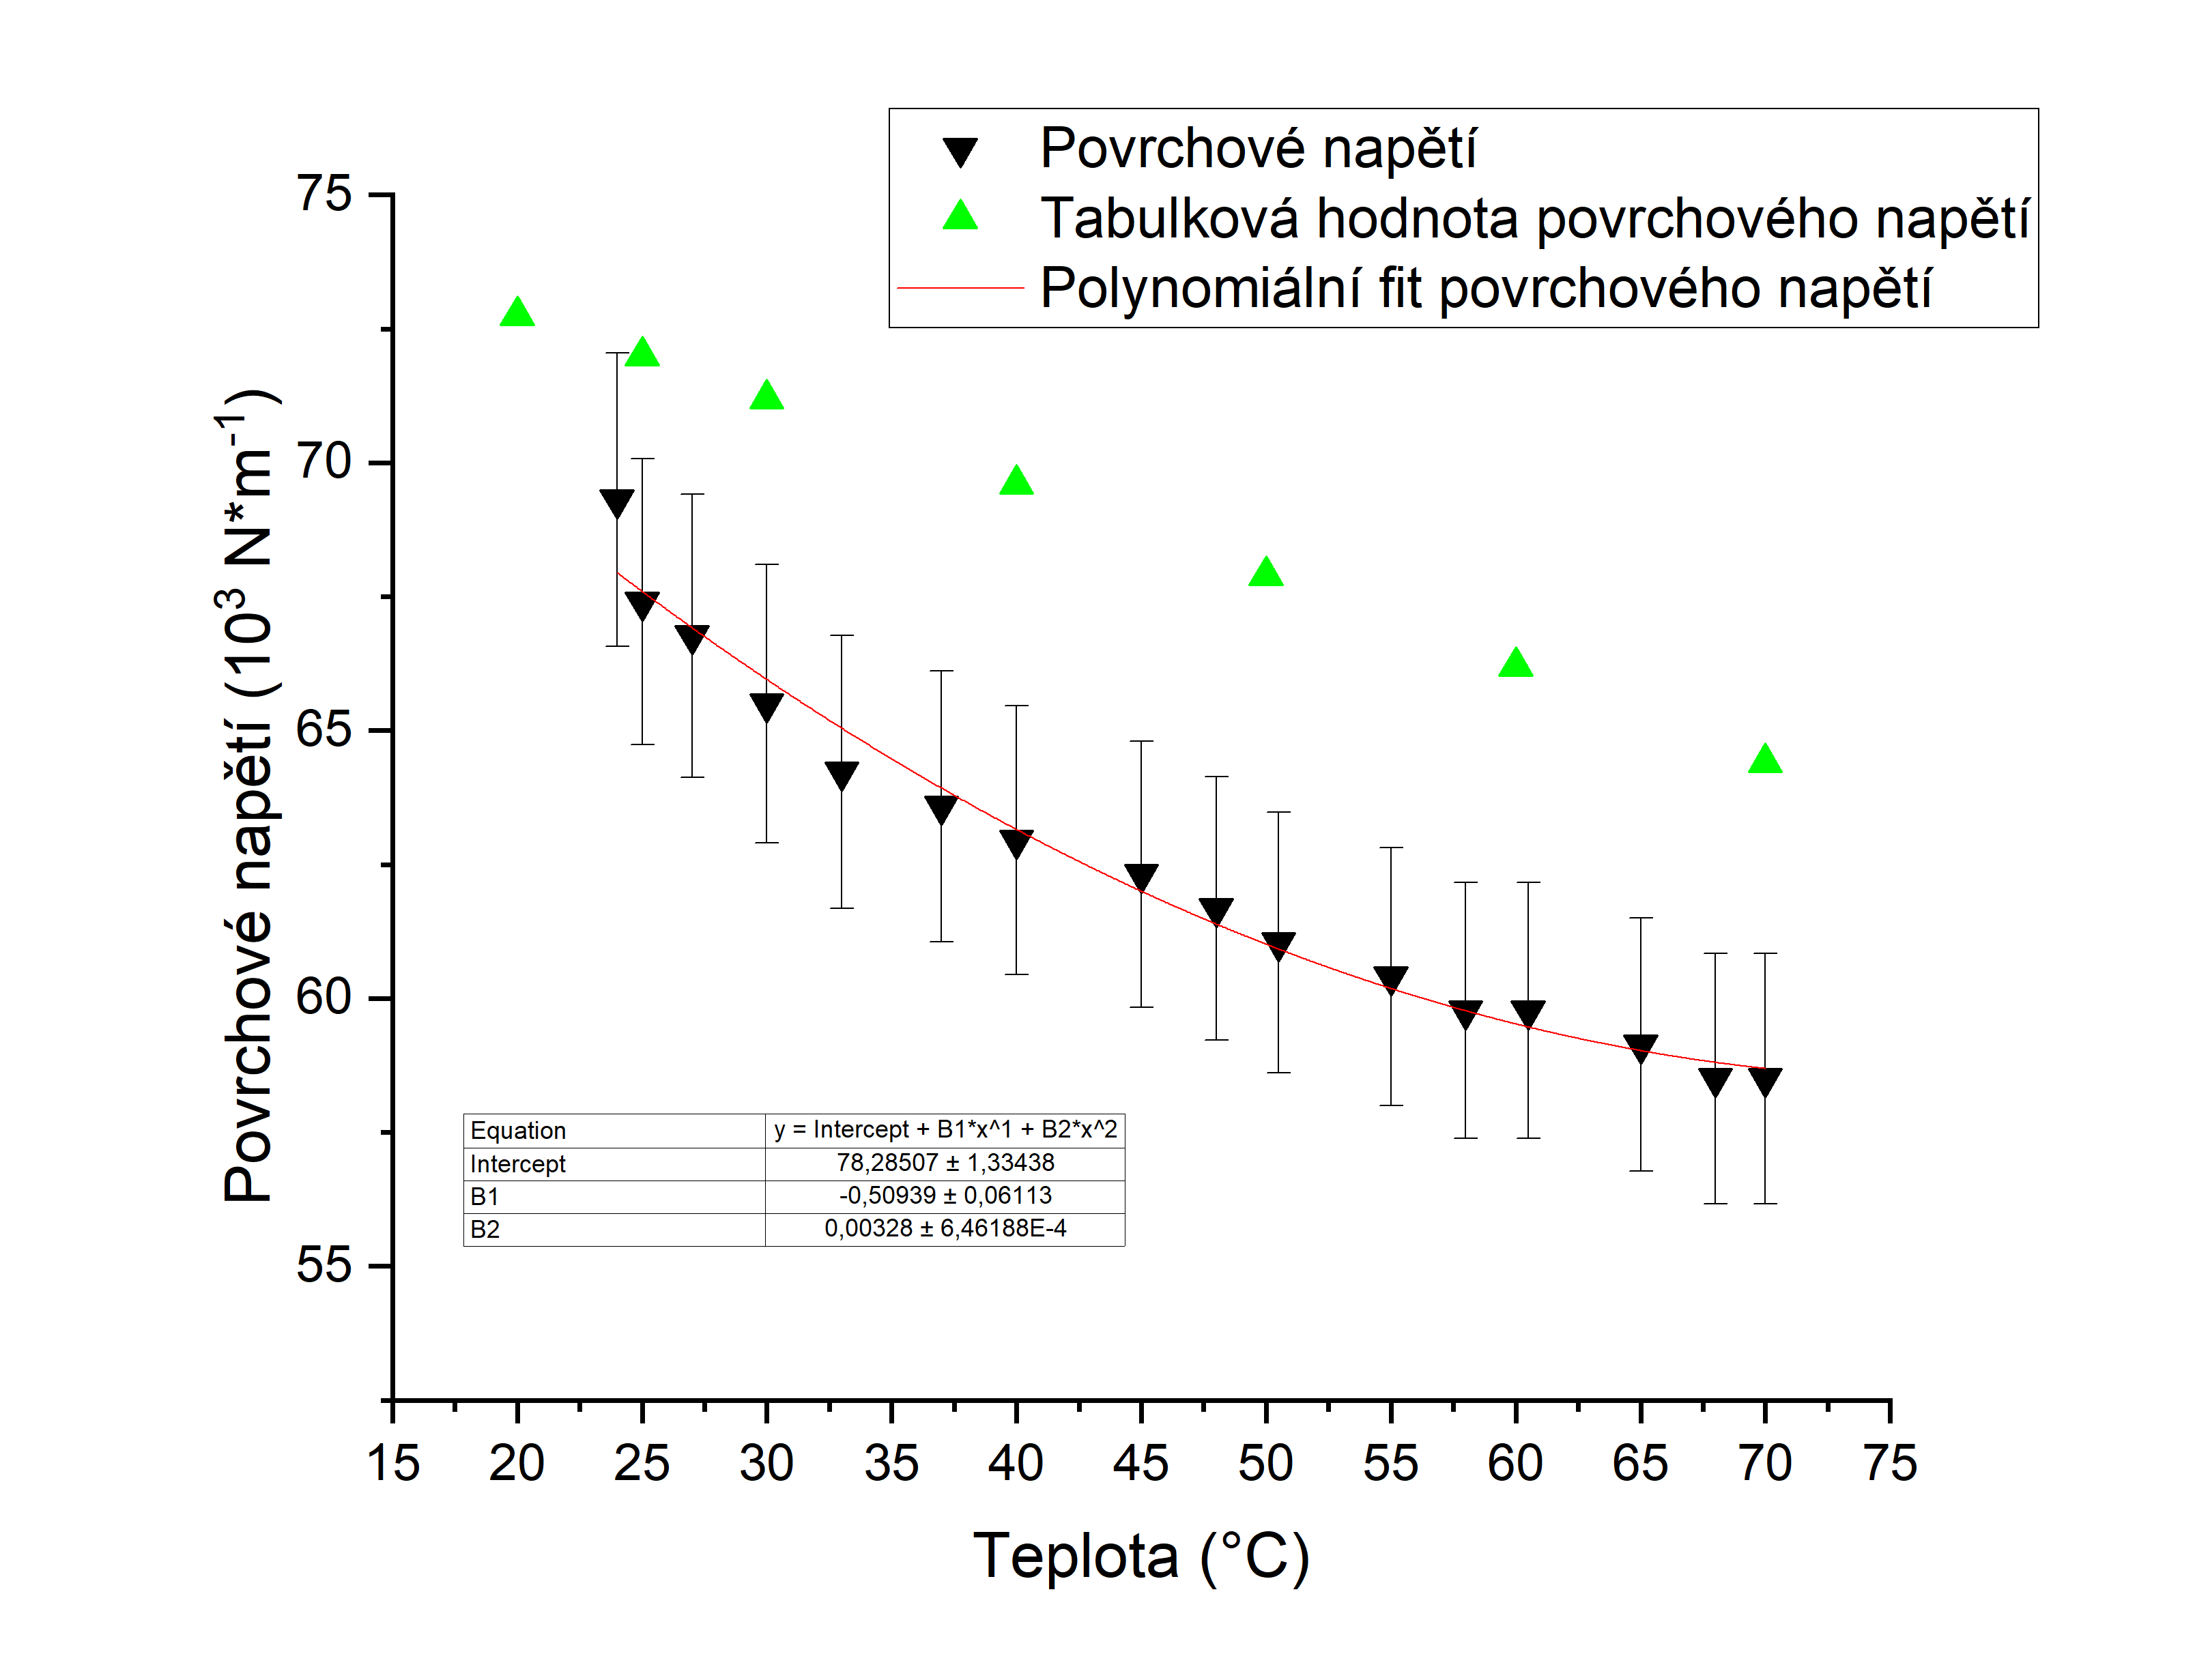
\includegraphics[width=1\linewidth]{14 - Studium teplotní závislosti povrchového napětí/Protokol - studium povrchového napětí/img/Závislost povrchového napětí na teplotě.png}
    \caption{Závislost povrchového napětí na teplotě}
    \label{fig:napeti-na-teplote}
\end{figure}

\newpage

Do grafu jsou zaneseny hodnoty povrchového napětí v závislosti na teplotě se svými chybovými úsečkami. Pro srovnání je zde zobrazena také závislost tabulovaných hodnot. Naměřená závislost byla dále fitována polynomiální funkcí se stupněm 2, tedy kvadratickou závislostí. Její předpis je $y = a + bx + cx^2$ s parametry

\begin{align*}
    a &= (78,3 \pm 1,3) N \cdot m^{-1}\\
    b &= (-0,5 \pm 0,1) N \cdot m^{-1} \cdot ^\circ C\\
    c &= (0,003 \pm 0,001) \cdot m^{-1} \cdot ^\circ C^2
\end{align*}



% ----------------------------------------------------------------------
%  Diskuse výsledků
% ----------------------------------------------------------------------			
\section{Diskuse výsledků}

Naše změřená závislost se ani v rámci chyby neshoduje s tabulkovými hodnotami, jak je vidět na grafu \ref{fig:napeti-na-teplote}. Při stejné teplotě se změřená teplota liší přibližně o $7 \cdot 10^{-3} N / m^{-1}$ oproti vyšší tabulkové hodnotě.

Důvodem odlišnosti výsledků může být zanedbaný hydrostatický tlak, přestože kapilára byla umístěna přibližně v 1 mm pod hladinou. Dále zde vstupuje nejistota určení teploty měřené kapaliny. Magnetické míchátko sice pracovalo v ohřívané kapalině, ale uvnitř baňky s měřenou kapalinou mohly vznikat oblasti s různými teplotami. Teploměr byl umístě v jedné poloze po celou dobu měření, proto měřil jen jedno místo. V kombinaci s nejistotou vlastního teploměru $\psi_T$ se zde může tato chyba projevit. Vlivem zpoždění zobrazení teploty na teploměru lze předpokládat, že skutečná teplota kapaliny je vyšší.

Posunutí celé závislosti by se dalo vysvětlit nepřesností určení poloměru bubliny, tedy poloměru kapiláry. Dalším sporným faktorem je určení momentu pro odečtení hodnoty změny tlaku. Záleží na rychlosti odtékání kapaliny z aspirátoru. To může ovlivnit neshodu mezi maximálním tlakem a minimálním poloměrem bubliny. Navíc toto odtékání kapalinu probíhá neustále i během měření jednotlivých hodnot.

Otázkou je také čistota měřené kapaliny, kterou jsme nijak neověřovali.

Při vyšších teplotách kapalina může ovlivnit parametry při povrchu kapaliny, například tlak v důsledku vypařování vody.

% ----------------------------------------------------------------------
%  Závěr
% ----------------------------------------------------------------------
\section{Závěr}

V tomto úkolu jsme změřili teplotní závislost povrchového napětí destilované vody $\sigma$ v rozsahu teplot od 23°C do 70°C metodou bublin. Měřenou závislost jsme znázornili graficky, do grafu vynesli chybové úsečky a tabulkové hodnoty. Závislost jsme aproximovali kvadratickou funkcí s parametry

\begin{align*}
    a &= (78,3 \pm 1,3) N \cdot m^{-1}\\
    b &= (-0,5 \pm 0,1) N \cdot m^{-1} \cdot ^\circ C\\
    c &= (0,003 \pm 0,001) \cdot m^{-1} \cdot ^\circ C^2
\end{align*}

Pro eliminaci rozdílu naměřené závislosti s tabulkovou bychom mohli požít různé poloměry trubic, nastavit ideální odtok kapaliny z aspirátoru a použít více teploměrů v měřené kapalině.